\documentclass[extra]{gji}
%~ \documentclass[extra, referee]{gji}

\usepackage[utf8]{inputenc}
\usepackage{timet}
\usepackage{amsmath}
\usepackage{graphicx}
%~ \usepackage{todonotes} % to make annotations on margins
\usepackage[disable]{todonotes} % to disable annotations on margins

\usepackage{url}
\usepackage[pdftex,colorlinks=true]{hyperref}
\hypersetup{
    allcolors=blue,
}


\begin{document}

\title[Variable Density Tesseroids]{
    Variable Density Tesseroids: Gravity fields calculation in spherical coordinates using variable densities in depth
}
\author[S.R. Soler, A. Pesce, L. Uieda and M.E. Gimenez]{
    Santiado R. Soler$^{1,2}$, Agustina Pesce$^{1,2}$, Leonardo Uieda$^3$ and Mario E. Gimenez$^{1,2}$ \\
    $^1$CONICET, Argentina. e-mail: santiago.r.soler@gmail.com\\
    $^2$Instituto Geofísico Sismológico Volponi, Universidad Nacional de San Juan, Argentina\\
    $^3$Universidade do Estado do Rio de Janeiro, Rio de Janeiro, Brazil
    }


\maketitle

\begin{summary}
Summary of this paper 
\end{summary}

\begin{keywords}
Satellite gravity??, Numerical modelling, Structure of the Earth, Gravity anomalies and Earth structure, Numerical approximations and analysis, spatial analysis??
\end{keywords}


\section{Introduction}

Lithosphere's density variation with depth has been studied for almost a century. 
On the first years \citet{Athy1930} obtained a decreasing exponential relation between both quantities by studying shale samples, while in the following decades other density functions have been proposed for different rock types \citep[e.g.,][]{Maxant1980, Rao1986, Rao1993, Rao1994}.
Furthermore, the density variation with depth has been taken into account in forward and inversion gravity models, mostly applied to grabens and basins \citep{Cordell1973, Rao1986, Cowie1990, Rao1993, Rao1994, Zhang2001, Welford2010}.

These forward gravity models have been developed for two or three dimensional bodies in cartesian coordinates that properly fit local scales applications.
Nevertheless, the latest satellite missions have provided us gravity measurements with global coverage, which allow geologists and geophysics to perform modelling and interpretation on regional scales.
This raises the importance of building forward models that reproduce the gravity anomalies for such scales.

The main issue that should be overcome is taking into account the curvature of the Earth, thus the forward model must be defined in spherical coordinates.
A common way to achieve this is to discretize the Earth in spherical prisms known as tesseroids, which are defined by pairs of latitude, longitude and radius boundaries (see Figure \ref{fig:tesseroid-uieda}).
Calculating the gravity fields generated by an arbitrary tesseroid on any external point involves the resolution of volume integrals that are generally approximated by numerical computations.
The literature offers two approaches: one involves Taylor series expansion \citep{Heck2007, Grombein2013} while the other makes use of Gauss-Legendre Quadrature (GLQ) \citep{Asgharzadeh2007, Uieda2016, Uieda2017}.

In order to develop a forward model that computes the gravity field generated by any tesseroid with arbitrary variable density, the Taylor series expansion is not well suited, because it would need to derive the series expansion terms for each density function.
On the other hand, the GLQ consists in approximating the integral by a weighted sum of the effect of point masses located at scaled nodes of the Legendre polynomials, where the density information is gathered into these weights.
Thus, this kind of numerical approximation allows to calculate the gravity fields for any density function without any other information but the function itself.

\begin{figure}
\centering
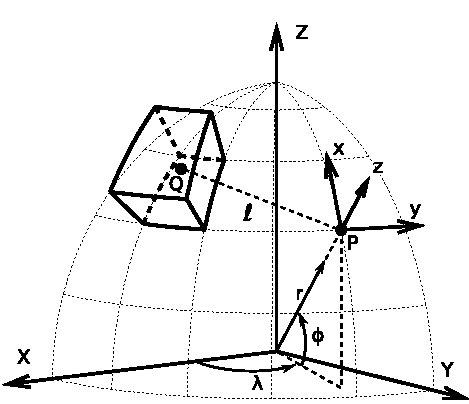
\includegraphics[width=0.9\linewidth]{figures/tesseroid-uieda.pdf}
\caption{
A spherical prism, also known as  Tesseroid, in a geocentric spherical coordinate system, with a computation point $P$ and its local north oriented Cartesian coordinate system. Picture made by \citet{Uieda2015}.
}
\label{fig:tesseroid-uieda}
\end{figure}

\citet{Uieda2016} developed a forward gravity model based on tesseroids with homogeneous densities using the GLQ approximation method.
It has been originally implemented through command line programs written in C programming language.
However, it has been ultimately ported to Python and included in the open-source library Fatiando a Terra \citep{Uieda2013} for geophysical modelling and inversion.

\citet{Ku1977} documented that the GLQ becomes less accurate when the computation point is closer to the tesseroid or for smaller GLQ order. 
Although the model developed by \citet{Uieda2016} uses a second order GLQ, it ensures the accuracy implementing a modified version of the adaptive discretization of \citet{Li2011}.
It consist in splitting the tesseroid into smaller ones when a certain distance-size ratio is lower than a predefined value ($D$) that controls the accuracy of the computation. 
\citet{Uieda2016} have also objectively obtained standard values of $D$ for gravity potential, gradients and tensor components comparing the fields generated by a spherical shell, which constitutes a special case of the volume integrals that has analytical solution \citep{LaFehr1991, Mikuska2006, Grombein2013}\todo{citar mas??}.

In addition, the varying density inside an arbitrary tesseroid introduces a new kind of error into the numerical approximation.
This encouraged us to develop a new density-based discretization algorithm that divides the tesseroid into smaller ones taking into account how the density function varies.
The number of subdivisions and thus the accuracy of the approximation will be controlled by a delta ratio $\delta$, a predefined value by the user.

We have enhanced the implementation of \citet{Uieda2016} with a new forward gravity model that allows us to compute the gravity fields generated by any tesseroid with an arbitrary density function on any external point.
It is based on the GLQ approximation, makes use of the modified distance-size discretization and the new density-based discretization algorithms that guarantee the accuracy even for high varying density functions.
It is written in Python and Cython languages, constituting an easy to use library that runs precompiled code for the more time consuming functions.
It also makes use of some previously existing classes and functions from Fatiando a Terra, what saved us time and allowed us to focus on the new enhancements.
Furthermore, we have the intention to include it into a future release of the Fatiando a Terra library in order to make its distribution and maintenance easier.

In order to ensure the accuracy of the numerical approximation, we have conducted similar tests as the one performed by \citet{Uieda2016} by comparing the results of the numerical model with the analytical solutions for a spherical shell with linear, exponential and discontinuous density.
Furthermore we had to derive the analytical expressions for these density functions.

In the following sections we will describe how the new algorithm works, its theoretical background and obtain default distance-size ratio and delta ratio values needed to get an acceptable accuracy in the numerical approximation.

%%%%%%%%%%%%%%%%%%%%%%%%%%%%%%%%%%%%%%%%%%%%%%%%%%%%%%%%%%%%%%%%%%%%%%%%%%%%%%

\section{Theory}

The spherical prisms known as tesseroids are mass elements defined in a geocentric spherical coordinate system bounded by a pair of parallels, a pair of  meridians, and two concentric spherical surfaces.
We define an external computation point $P(r, \phi, \lambda)$ where the gravity fields generated by the tesseroid are going to be calculated with respect to the local north oriented Cartesian coordinate system located at $P$.
In the special case of homogeneous density, the gravity potential, its gradient and the Marussi tensor components can be calculated through the integrals obtained by \citet{Grombein2013} \citep[for same notation as the one we will use, see][]{Uieda2016}.

In our case, we will assume that the tesseroid has an arbitrary variable density in depth, i.e. only depends on the radius spherical coordinate.
Thus, the integrals for the gravity fields are slightly modified:

\begin{equation}
    V(r,\phi,\lambda) = G
    \int\limits_{\lambda_1}^{\lambda_2}
    \int\limits_{\phi_1}^{\phi_2}
    \int\limits_{r_1}^{r_2}
    \frac{\rho(r')}{\ell} \kappa \,  dr' d\phi' d\lambda',
\label{eq:tesseroid-pot}
\end{equation}
\begin{equation}
    g_{\alpha}(r,\phi,\lambda) = G
    \int\limits_{\lambda_1}^{\lambda_2}
    \int\limits_{\phi_1}^{\phi_2}
    \int\limits_{r_1}^{r_2}
    \rho(r') \frac{\Delta_\alpha}{\ell^3}
    \kappa \, dr' d\phi' d\lambda',
\label{eq:tesseroid-grav}
\end{equation}
\begin{equation}
    g_{\alpha\beta}(r,\phi,\lambda) = G
    \int\limits_{\lambda_1}^{\lambda_2}
    \int\limits_{\phi_1}^{\phi_2}
    \int\limits_{r_1}^{r_2}
    \rho(r') I_{\alpha\beta} \, \kappa \, dr' d\phi' d\lambda' ,
    \label{eq:tesseroid-tensor}
\end{equation}

\noindent where

\begin{equation}
    I_{\alpha\beta} =
    \left(
        \frac{3\Delta_{\alpha} \Delta_{\beta}}{\ell^5} -
        \frac{\delta_{\alpha\beta}}{\ell^3}
    \right) ,
    \label{eq:tesseroid-tensor-kernel}
\end{equation}

\noindent $\alpha, \beta \in \{x, y, z\}$,
$\rho(r')$ is the density function that depends on the radial coordinate,
$\delta_{\alpha\beta}$ is Kronecker's delta,
$G = 6.674\times10^{-11}\, \text{m$^3$kg$^{-1}$s$^{-1}$}$ is the gravitational constant and

\begin{equation}
    \Delta_x = r'[\cos\phi\sin\phi' - \sin\phi\cos\phi'
               \cos(\lambda' - \lambda)],
\end{equation}
\begin{equation}
    \Delta_y = r' \cos \phi' \sin(\lambda' - \lambda),
\end{equation}
\begin{equation}
    \Delta_z = r' \cos \psi - r,
\end{equation}
\begin{equation}
    \kappa = {r'}^2 \cos \phi',
\end{equation}
\begin{equation}
    \ell = \sqrt{{r'}^2 + r^2 - 2 r r' \cos \psi},
\label{eq:ell}
\end{equation}
\begin{equation}
    \cos\psi = \sin\phi\sin\phi' + \cos\phi\cos\phi'
                 \cos(\lambda' - \lambda).
\label{eq:cospsi}
\end{equation}


According to \citet[p.~390]{Hildebrand1987}, we can approximate any integral in the interval $[-1, 1]$ using a $N$th order GLQ, i.e. by a weighted sum of the integration kernel evaluated on the roots of the $N$th Legendre polynomial:

\begin{equation}
    \int\limits_{-1}^1 f(x) dx \approx \sum_{i=1}^N W_i f(x_i),
\end{equation}

\noindent where $x_i$ are the roots of the $N$th Legendre polynomial $P_N(x)$ and $W_i$ are the weights of each term:

\begin{equation}
    W_i = \frac{2}{(1-x_i^2)[P_N^\prime(x_i)]^2},
\end{equation}

\begin{equation}
    P_N(x_i) = 0, \quad \forall i = {1,\dots,N}.
\end{equation}

In case of an integration defined on a arbitrary interval, e.g. $[a,b]$, we can scale the nodes and perform a similar approximation:

\begin{equation}
    \int\limits_a^b f(x) dx \approx \frac{b-a}{2} \sum_{i=1}^N W_i f(x_i^s),
\label{eq:glq-scaled}
\end{equation}

\noindent where $x_i^s$ is the scaled $x_i$ root into the $[a,b]$ interval, also called nodes of the quadrature:

\begin{equation}
    x_i^s = \frac{b-a}{2} x_i + \frac{b+a}{2}.
\end{equation}

\noindent For example, if we use a second order GLQ, the roots of the $P_2(x)$ Legendre polynomial and its corresponding weights are $x_i = \pm 0.577350269$ and $W_i = 1$.

Our intention is to use GLQ to approximate the volume integrals from equations \ref{eq:tesseroid-pot}-\ref{eq:tesseroid-tensor}. 
When tesseroids have variable densities, we can write the integral kernels as the product of a certain function $g$ and the density function:

\begin{equation}
    f(r', \phi', \lambda') = \rho(r') g(r', \phi', \lambda'),
\end{equation}

\noindent and then apply the quadrature to every integral corresponding to each spherical coordinate, obtaining a similar expression to the one shown by \citet{Asgharzadeh2007} and \citet{Uieda2016}:

\iftwocol{
\begin{equation}
    \begin{split}
        \iiint\limits_\Omega \rho(r') g(r', \phi', \lambda') 
        d\Omega \approx& \\
        A 
        \sum\limits_{i=1}^{N^r}
        \sum\limits_{j=1}^{N^\phi}
        \sum\limits_{k=1}^{N^\lambda}
        & W_i^r W_j^\phi W_k^\lambda \rho(r_i) g(r_i, \phi_j, \lambda_k),
    \end{split}
\label{eq:glq-var-dens}
\end{equation}
}{
\begin{equation}
    \iiint\limits_\Omega \rho(r') g(r', \phi', \lambda') d\Omega \approx
    A 
    \sum\limits_{i=1}^{N^r}
    \sum\limits_{j=1}^{N^\phi}
    \sum\limits_{k=1}^{N^\lambda}
    W_i^r W_j^\phi W_k^\lambda \rho(r_i) g(r_i, \phi_j, \lambda_k),
\label{eq:glq-var-dens}
\end{equation}
}

\noindent where

\begin{equation}
    A = 
    \frac{(\lambda_2 - \lambda_1)(\phi_2 - \phi_1)(r_2 - r_1)}{8}.
\end{equation}

In the same way as for an homogeneous density, we can observe from equation \ref{eq:glq-var-dens} that the GLQ approximates the gravity fields of a tesseroid as the ones generated by point masses located at the nodes of the Legendre polynomials.
Nevertheless, in the variable density case, the information of the density function is summarised into the weights of the sum by taking into account only the values it assumes on those nodes.
Although this may sound discouraging, we intent to prove otherwise and show that this method, along with well fitted discretization algorithms, approximates the gravity fields with good accuracy.\todo{no se si poner esta ultima oracion}


\subsection{Analytical Solutions for Spherical Shell}

The integrals that define the gravity fields in equations \ref{eq:tesseroid-pot}-\ref{eq:tesseroid-tensor} have analytical solutions for the exceptional case of a spherical shell with homogeneous density \citep{Mikuska2006,Grombein2013}.
In order to test the accuracy of their approximations, \citet{Uieda2016} and \citet{Grombein2013} compared their numerical models (tesseroids with homogeneous density) with these analytical solutions.

In case of variable density tesseroids, the comparison must obviously be made with a variable density spherical shell, whose analytical solution will depend on the chosen density function.
Because the literature has not offered it yet, we had to develop it ourselves. \todo{ no se si ponerlo asi}

Lets consider a spherical shell with inner and outer radii $R_1$ and $R_2$, respectivetly, whose density depends on the radius spherical coordinate (Figure \ref{fig:spherical-shell}).
The gravity potential generated by the shell on an arbitrary external point $Q(0,0,r)$, located along the $z$ axe at a distance $r$ from the origin, can be written as follows:

\begin{figure}
\centering
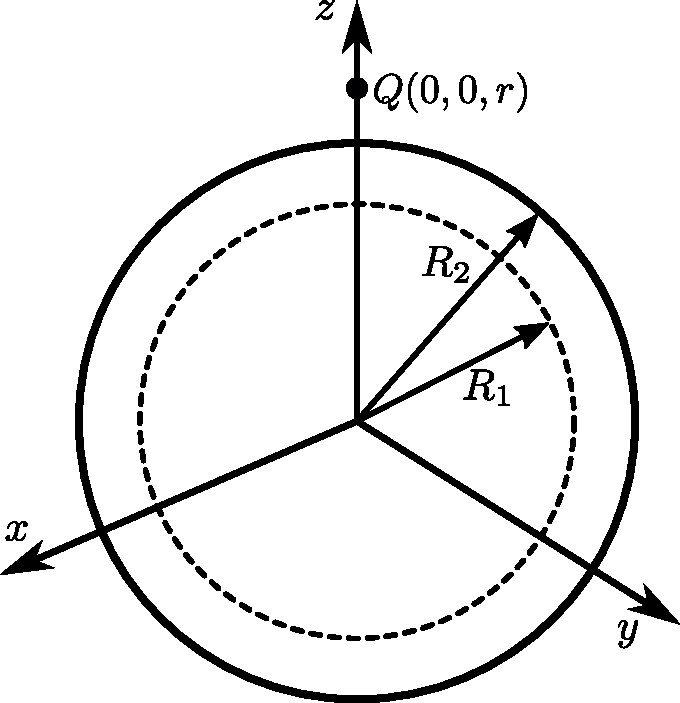
\includegraphics[width=0.7\linewidth]{figures/spherical-shell.pdf}
\caption{
Spherical shell with inner and outer radii $R_1$ and $R_2$, respectively.
The computation point $Q$ is located in the $z$ axe at a distance $r$ from the centre of the shell.
For practical purposes we will assume that $Q$ is outside the outer radii, i.e. $r > R_2$.
}
\label{fig:spherical-shell}
\end{figure}

\begin{equation}
    V_\text{sh}(r) = G 
    \int\limits_0^{2\pi}
    \int\limits_{-\frac{\pi}{2}}^\frac{\pi}{2}
    \int\limits_{R_1}^{R_2}
    \frac{\rho(r')}{\ell} {r'}^2 \cos\phi' \, 
    dr' d\phi' d\lambda',
\end{equation}

\noindent where $\ell$ is defined in equation \ref{eq:ell}.
The computation point $Q$ is located at latitude $\phi=90^\circ$, so $\ell$ and $\cos\psi$ (defined in equation \ref{eq:cospsi}) get simplified:

\begin{equation}
    \cos\psi = \sin\phi', \quad
    \ell = \sqrt{r'^2 + r^2 - 2 r r' \sin\phi'}.
\end{equation}

Due to the rotational symmetry along the $z$ axe, the integration in $\lambda'$ is straightforward:

\begin{equation}
    V_\text{sh}(r) = 2\pi G 
    \int\limits_{-\frac{\pi}{2}}^\frac{\pi}{2}
    \int\limits_{R_1}^{R_2}
    \frac{\rho(r') {r'}^2 \cos\phi'}{\sqrt{r'^2 + r^2 - 2 r r' \sin\phi'}}
    \, dr' d\phi',
\end{equation}

\noindent while the integration in $\phi'$ can be performed independently of the density function.
Taking into account the following integral:

\begin{equation}
    \int \frac{\cos \phi}{\sqrt{a - b \sin \phi}} \, d\phi =
    -\frac{2}{b} \sqrt{a - b \sin \phi} + C,
\end{equation}

\noindent the potential can be written as follows:

\iftwocol{
\begin{equation}
    \begin{split}
        V_\text{sh}(r) = 2\pi G
        \int\limits_{R_1}^{R_2}
        \Big[ & \sqrt{r^2 + r'^2 + 2rr'} - \\
        & \sqrt{r^2 + r'^2 - 2rr'}
        \Big] \frac{r'\rho(r')}{r} \, dr'.
    \end{split}
\label{eq:shell-pot-sqrts}
\end{equation}
}{
\begin{equation}
    V_\text{sh}(r) = 2\pi G
    \int\limits_{R_1}^{R_2}
    \Big[ \sqrt{r^2 + r'^2 + 2rr'}  -
    \sqrt{r^2 + r'^2 - 2rr'} 
    \Big] \frac{r'\rho(r')}{r} \, dr'.
\label{eq:shell-pot-sqrts}
\end{equation}
}

For our purposes we can assume that the computation point $Q$ is outside the outer radii, i.e. $r>R_2$ ($R_2 \geq r'$), and simplify the square roots in equation \ref{eq:shell-pot-sqrts}:

\begin{equation}
    \sqrt{r^2 + r'^2 + 2rr'} = |r + r'| = r + r',
\end{equation}
\begin{equation}
    \sqrt{r^2 + r'^2 - 2rr'} = |r - r'| = r - r',
\end{equation}

\noindent what leads to the following expression of the potential of the spherical shell:

\begin{equation}
    V_\text{sh}(r) = \frac{4\pi G}{r}
    \int\limits_{R_1}^{R_2} {r'}^2 \rho(r') \, dr'.
\label{eq:shell-pot}
\end{equation}

The equation \ref{eq:shell-pot} allows to easily obtain the exact gravity potential generated by a spherical shell with a variable density in depth on any outside point located in the $z$ axe.
Due to the rotational symmetry along any axe that passes through the centre of the shell, the integral in equation \ref{eq:shell-pot} reproduces the gravity potential field on any outside point at distance $r$ from the its centre.

The gradient and the Marussi tensor derived from potentials that depends solely on $r$ have only a few non zero components: the vertical component of the gradient ($g_z$) and the diagonal components of the tensor ($g_{xx}$, $g_{yy}$, $g_{zz}$).
They can be easily obtained as \citet{Grombein2013} does, even for any arbitrary density function $\rho(r')$:

\begin{equation}
    g_z = \frac{V_\text{sh}(r)}{r},
\end{equation}
\begin{equation}
    g_{xx} = g_{yy} = -\frac{V_\text{sh}(r)}{r^2}, \quad
    g_{zz} = \frac{2V_\text{sh}(r)}{r^2}.
\end{equation}

For practical purposes we are going to obtain the gravity potential for three different functions from the perspective of their variation in $r'$: a linear and an exponential density function.


\subsubsection{Linear Density}

If the density of the spherical shell is a linear function on the radial coordinate, i.e.:

\begin{equation}
    \rho(r') = ar' + b,
\end{equation}

\noindent then the gravity potential generated on any computation point at distance $r$ from its centre can be obtained from the following expression:

\begin{equation}
    V_\text{sh}^\text{lin}(r) = \pi G \left[ 
    a \frac{R_2^4 - R_1^4}{r} +
    b \,\frac{4}{3} \frac{R_2^3 - R_1^3}{r} \right].
    \label{eq:shell-pot-linear}
\end{equation}

The second term on equation \ref{eq:shell-pot-linear} reproduces the potential generated by a spherical shell with homogeneous density $\rho = b$ \citep{Mikuska2006,Grombein2013}.
So it can be read as the combination of a spherical shell with the later homogeneous density and the same shell with variable density $\rho(r') = ar'$.


\subsubsection{Exponential Density}

If, on the other hand, the spherical shell has an exponential density in the radial coordinate,

\begin{equation}
    \rho(r') = Ae^{-(r' - \Delta h)/b},
\end{equation}

\noindent the potential can be written as follows:

\iftwocol{
\begin{equation}
    \begin{split}
        V_\text{sh}^\text{exp}(r) = \frac{4\pi G}{r} 
        Ab \, e^\frac{\Delta h}{b}
        \Big[
        & (R_1^2 + 2R_1 b + 2b^2)e^{-\frac{R_1}{b}} - \\
        & (R_2^2 + 2R_2 b + 2b^2)e^{-\frac{R_2}{b}}
        \Big].
    \end{split}
\label{eq:shell-pot-exp}
\end{equation}
}{
\begin{equation}
    V_\text{sh}^\text{exp}(r) = \frac{4\pi G}{r} 
    Ab \, e^\frac{\Delta h}{b}
    \Big[
    & (R_1^2 + 2R_1 b + 2b^2)e^{-\frac{R_1}{b}} - \\
    & (R_2^2 + 2R_2 b + 2b^2)e^{-\frac{R_2}{b}}
    \Big].
\label{eq:shell-pot-exp}
\end{equation}
}

%%%%%%%%%%%%%%%%%%%%%%%%%%%%%%%%%%%%%%%%%%%%%%%%%%%%%%%%%%%%%%%%%%%%%%%%%%%%%%%

\section{Implementation}

We have developed a Python library that computes the gravity fields generated by any Tesseroid with variable density in depth.
It is freely available under the BSD 3-clause open-source library and can be downloaded from the following repository: \todo{agregar repo, vale la pena poner el link?}

This new library is based on the preexisting code developed by \citet{Uieda2016} (and included in Fatiando a Terra v.0.5, \citet{Uieda2013}) that is able to compute only the gravitational effects of tesseroids with homogeneous density.
\citet{Uieda2016} have optimised the more time consuming functions through the Numba compiler.
In contrast, we have decided to develop our new library in Cython language due to difficulties when passing a Python function as argument to precompiled Numba methods, keeping the homogeneous tesseroid calculation and adding the new variable density computations.
The Cython language is a superset of Python language that allows to generate efficient C code through the Cython compiler, producing a library whose functions can be called from regular Python code.

Moreover, this new software is compatible with the preexisting open-source library Fatiando a Terra and its usage is very similar to the one for homogeneous tesseroids:

\begin{enumerate}
\renewcommand{\theenumi}{(\arabic{enumi})}
    \item Define a single tesseroid (or a set of several tesseroids) with the Fatiando a Terra classes.
    \item Add a predefined Python density function to the tesseroid (or to each tesseroid in the set).
    \item Calculate the desired gravity field (potential, gradient or tensor components) on any set of computation points.
\end{enumerate}

In a more detailed way, the new library approximates the gravitational effect of each tessseroid through the GLQ, and increases its accuracy with the modified version of the adaptive discretization algorithm, original developed by \citet{Li2011} and improved by \citet{Uieda2016}.

In addition, we had to develop a new density-based discretization algorithm in order to decrease a new type of error in the numerical approximation caused by high variations in the density functions.
It is intended to work together with the preexisting modified adaptive discretization algorithm.


\subsection{Modified Adaptive Discretization Algorithm}

From equation \ref{eq:glq-var-dens} we saw that the GLQ approximates the volume integrals as the gravitational effect of $N_\lambda N_\phi N_r$ point masses, where $N_i$ are the orders of the quadrature for the integral on each coordinate, with $i \in \{ \lambda, \phi, r \}$.
If we set the GLQ orders to fixed values, it's easy to conclude that the nearer the computation point is to the tesseroid, the accuracy of the approximation is reduced and the point masses effect becomes more noticeable than the tesseroid we want to approximate.
A more complete analysis of this conclusion can be found in \citet{Ku1977, Li2011, Uieda2016}.

Instead of increasing the GLQ orders to improve the accuracy, what leads to a more time consuming computation, adaptive discretization algorithms have been applied in previous works \citep{Li2011, Uieda2016}.
They essentially consist in dividing the tesseroid based on a ratio between the distance from its geometric centre to the computation point and its dimensions.

In order to make the computation more efficient, we use only second order GLQ for each integration while we ensure the accuracy of the method through the application of the modified adaptive discretization algorithm developed by \citet{Uieda2016}.
The modifications made by \citet{Uieda2016} to the original adaptive discretization method \citep{Li2011} can be summed up in:
(1) a faster calculation of the distance from the computation point to the tesseroid and 
(2) the application of a stack based algorithm that speeds up the computation and gives more control over the recursion step.

More specifically, \citet{Uieda2016} redefined the dimensions of an arbitrary tesseroid: $L_\lambda$, $L_\phi$ and $L_r$. The former ones are the arc-distances measured along its top surface while $L_r$ is the difference between the radii of the top and bottom surfaces.

The adaptive discretization algorithm starts by checking that the following inequality is satisfied:

\begin{equation}
    \frac{d}{L_i} \geq D,
\label{eq:distance-size-ratio}
\end{equation}

\noindent where $i \in \{\lambda, \phi, r\}$, $d$ is the distance between the geometric centre of the tesseroid and the computation point, and $D$ is a predefined value called distance-size ratio.
If the inequality \ref{eq:distance-size-ratio} is not held for any spherical coordinate, then the tesseroid must be divided by half in that direction.
A more complete description of the modified adaptive discretization algorithm can be found in \citet{Uieda2016}.
On the contrary, if the inequality is satisfied, the algorithm computes the desired gravity field using the GLQ approximation.

In summary, the distance-size ratio $D$ determines indirectly how many times the tesseroids will be divided, and therefore regulates both the accuracy of the algorithm and its computation time.
In this way the modified version of the adaptive discretization algorithm efficiently improves its accuracy and gives the user more control over the computation: it allows to stop the division of the tesseroids when their dimensions are lower than a certain value (e.g. less than 10 cm), in which case it does not modifies significantly the desired gravitational field.

On the other hand, the value assigned to the distance-size ratio $D$ cannot be easily related to the error of the approximation, thus the choice of the value of $D$ to get an acceptable accuracy must be objectively determined beforehand.
In order to overcome this, \citet{Uieda2016} compared the numerical computation with the analytical solution for a spherical shell with homogeneous density.

We will perform similar tests, but now with variable density spherical shell.
From the infinite density functions that can be proposed, we have chosen three characteristic ones: a linear, an exponential and a discontinuous function.

\subsection{Density-based Discretization Algorithm}

High variations in the density function of an arbitrary tesseroid introduces a new type of error into the numerical approximation: only a few point masses would not reproduce the effect of this kind of variations.
The modified version of the adaptive discretization algorithm may help in reducing this kind of error, but as it only takes into account the dimensions of the tesseroid and the distance to the computation point, it's not well suited to fully perform this task.

In order to overcome this, we developed a complementary discretization algorithm that takes into account the variation of the density inside the tesseroid.
Basically, it subdivides any tesseroid on the radial direction on the depth at which the \emph{maximum density variation} takes place.

Specifically, the algorithm consists in the following steps:

\begin{enumerate}
\renewcommand{\theenumi}{(\arabic{enumi})}
    \item Normalise the density function to the [0, 1] interval,
    \item Compute the absolute difference between the normalised density and a linear function that assumes the same values on the top and bottom radii that this normalised density.
    \item If the maximum of the absolute difference is greater that a predefined delta ratio ($\delta$), then the tesseroid will be subdivided on the radius at which this maximum takes place. Otherwise, the tesseroid won't be split.
\end{enumerate}

First we need to normalise the density function such as it assumes the values of 0 and 1 on the boundary radii ($R_1$, $R_2$), depending at which radius the original density function is maximum.
We call this normalised density $\rho_n(r')$ and we calculate it as follows:

\begin{equation}
    \rho_n(r') = \frac{\rho(r') - \rho_1}{\rho_2 - \rho_1},
\end{equation}
\noindent where
\begin{equation}
    \rho_1 = \text{min}\{ \rho(R_1), \rho(R_2) \}, \quad
    \rho_2 = \text{max}\{ \rho(R_1), \rho(R_2) \}.
\end{equation}

Secondly, we must define a linear function $\rho_l(r')$ that assumes the same values of the normalised density $\rho_n(r')$ on the boundary radii:

\begin{equation}
    \rho_l(r') =
    \frac{ \rho_n(R_2) - \rho_n(R_1) }{ R_2 - R_1 } (r' - R_1) + \rho_n(R_1),
\end{equation}

\noindent and compute the absolute difference between this linear function and the normalised density:

\begin{equation}
    \Delta \rho (r') = | \rho_n(r') - \rho_l(r') |.
\end{equation}

Finally, if the maximum of the absolute difference if greater than a predefined delta ratio $\delta$ we will divide the tesseroid on the radius at which this maximum takes place ($R_\text{max}$):

\begin{equation}
    \text{max}\{ \Delta \rho(r') \} > \delta,
    \label{eq:delta-density}
\end{equation}
\begin{equation}
    \text{max}\{ \Delta \rho(r') \} = \Delta \rho(R_\text{max}),
\end{equation}

\noindent obtaining a pair of smaller tesseroids with the same longitude and latitude boundaries.

In case that the original density function assumes the same value at both boundary radii, the procedure is the same except that the constants $\rho_1$ and $\rho_2$ are redefined as follows:

\begin{equation}
    \rho_1 = \text{min}\{ \rho(r') \}, \quad
    \rho_2 = \text{max}\{ \rho(r') \}.
\end{equation}

If on the contrary the inequation \ref{eq:delta-density} is not held, then the tesseroid will not be subdivided.
The same happens if the density function is constant or if the tesseroid radius dimension is bellow the threshold of 1mm.
On the first case due to the fact that the density-based discretization algorithm is not needed, and on the second one because smaller tesseroids will not introduce meaningful increases in the accuracy of the computation.

This algorithm can be subsequently applied to every subdividing tesseroid, until the inequation \ref{eq:delta-density} is not held or the subdivisions are smaller than 1mm.
This two conditions guarantee that the algorithm is finite, i.e. it does not fall into an infinite loop. \todo{chequear esta oracion}
Once this conditions are met, every subdividing tesseroid is subjected to the modified adaptive discretization algorithm and the GLQ in order to compute the gravity field generated by it.

It's easy to see that the delta ratio indirectly controls how many times the tesseroids will be subdivided based on the variation of the density function. Therefore it controls the accuracy involving the numerical error that the density variation introduces and also the computation time.
This raises the need to determine a maximum value of $\delta$ that ensures an acceptable accuracy while minimising the computation time.
We will perform this determination with the same methodology as the one applied to the $D$ ratio: compare the numerical model with the analytical solutions for a spherical shell.


\subsection{Algorithm summary}

When computing any gravity field generated by an arbitrary tesseroid on a specific computation point, the new software:

\begin{enumerate}
    \renewcommand{\theenumi}{(\arabic{enumi})}
    \item Applies the density-based discretization algorithm in case of variable density producing subdivisions of the original tesseroid,
    \item Applies the modified adaptive discretization algorithm for each subdivision, generating a set of smaller tesseroids,
    \item Computes the desired gravity field for every small tesseroid through the GLQ approximation (equation \ref{eq:glq-var-dens}).
\end{enumerate}

These steps are applied for each computation point, adding the contribution of each tesseroid to the resulting gravity field.

%%%%%%%%%%%%%%%%%%%%%%%%%%%%%%%%%%%%%%%%%%%%%%%%%%%%%%%%%%%%%%%%%%%%%%%%%%%%%%%

\section{Determination of distance-size ratio}

In order to determine the minimum value for the distance-size ratio $D$ such the numerical approximation achieves an acceptable accuracy we have compared the numerical model with the analytical solutions for a spherical shell with variable density for three special cases: a linear, an exponential and a discontinuous density function.
The first one constitutes the simplest variation, while the second one represents a higher varying function. The later one tries to emulate a contact between two different media (e.g. crust and mantle interface).

We approximated the spherical shell by a mesh of $30^\circ \times 30^\circ$ tesseroids and calculated the gravity potential, the vertical component of the gradient ($g_z$) and the diagonal components of the Marussi tensor ($g_{xx}$, $g_{yy}$, $g_{zz}$) on four different grids: (1) a grid located at the pole, (2) another one on the Equator, (3) one located at satellite height and (4) a big grid of $30^\circ \times 30^\circ$.
More information about this grids can be found on Table \ref{tab:grids}.

We computed these gravity fields on every point of the four grids for different values of $D$, ranging from 0.5 to 10 with a step of 0.5.
Then we calculated the maximum difference between these results and the value that the analytical solution assumes at the same height.

Because the gravity fields generated by a tesseroid are approximated by the effect of point masses, the numerical results may vary between computation points at same height but at different latitude or longitude.
That's why we choose for comparison the maximum difference between the results on every point of the grid and the analytical solution.

Moreover, we did not apply the density-based discretization algorithm in these tests in order to isolate the behaviour of the adaptive discretization algorithm.

Finally, we set the acceptable value of $D$ if the corresponding error of the numerical approximation is lower than 0.1\%.

\begin{table}
\caption{
    Description of the synthetic grids on which the comparison of the numerical model against the analytical solutions for a spherical shell was done. This collection of grids tries to include every possible scenario on which the numerical model can present a different behaviour depending on the size of the grid, its location or its height over the Earth surface. Every grid consists in a set of 10$\times$10 points.
}
\label{tab:grids}
\begin{tabular}{lcccc}
    Grid & Size & Lat. extension & Lon. extension & Height \\ \hline
    Pole & $1^\circ \times 1^\circ$ & $89^\circ - 90^\circ$ & $0^\circ - 1^\circ$ & 2km \\
    Equator & $1^\circ \times 1^\circ$ & $0^\circ - 1^\circ$ & $0^\circ - 1^\circ$ & 2km \\
    Satellite & $1^\circ \times 1^\circ$ & $89^\circ - 90^\circ$ & $0^\circ - 1^\circ$ & 260km \\
    Big Grid & $30^\circ \times 30^\circ$ & $60^\circ - 90^\circ$ & $0^\circ - 30^\circ$ & 2km \\
\end{tabular}
\end{table}


\subsection{Linear Density}
Firstly,  we proposed a spherical shell with linear density in such way that it assumes 2670~kg/m$^3$ on the surface of the Earth and 3300~kg/m$^3$ at the inner radius:

\begin{equation}
    \rho(r') = ar' + c,
    \label{eq:density-linear}
\end{equation}
\noindent with 
\begin{equation}
    a = -\frac{3300\text{kg/m$^3$} - 2670\text{kg/m$^3$}}{R_2 - R_1},
\end{equation}
\begin{equation}
    c = \frac{3300\text{kg/m$^3$} - 
        2670\text{kg/m$^3$}}{R_2 - R_1} R + 
        2670\text{kg/m$^3$},
\end{equation}

\noindent where $R$ = 6378.137 km is the mean Earth radius.

Then we computed the difference between the numerical model with its corresponding analytical solution (equation \ref{eq:density-linear}) for a thick and a thin spherical shell of 1km and 35km of thickness, respectively.

In Figures \ref{fig:D-linear-thin} and \ref{fig:D-linear-thick} we can see the results for the potential, the vertical component of the gradient $g_z$ and the $g_{zz}$ component of the Marussi tensor.
Because the other two diagonal components of the tensor show similar results as the ones obtained for the $g_{zz}$, we exclude them from the figure, although they can be found in the repository. \todo{chequear}

For the linear density case, we can observe that the calculation of the potential and the $g_z$ component of its gradient needs a value of $D=1$ and $D=2$, respectively, in order to ensure an accuracy of 0.1\%.
On the other hand, the $g_{zz}$ computations show a noticeable difference between the thin and the thick shell: the first one needs a value of $D$ equal to 8 while the later only a $D$ of 3.5.
We will keep the more conservative result of $D$ equal to 8 in case of computing the Marussi tensor components in case of a linear density tesseroid.

It's worth to remember that the density-based discretization algorithm is not applied for linear density function comparisons, thus the adaptive discretization algorithm is the only mechanism that controls the accuracy of the approximation.

\begin{figure}
\centering
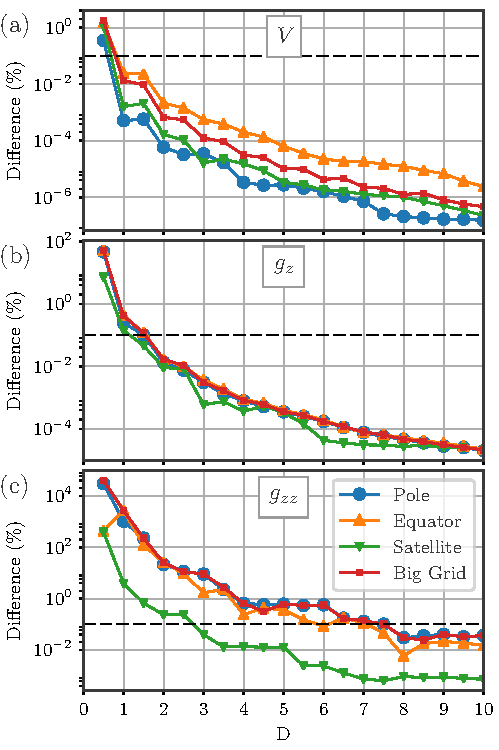
\includegraphics[width=0.9\linewidth]{figures/linear-D-thin.pdf}
\caption{
    Differences between the gravity fields generated by the numerical model and the analytical solution for a thin spherical shell of 1km of thickness with the linear density defined on equation \ref{eq:density-linear}. The computations were performed on the four grids described in Table \ref{tab:grids}, for different values of the distance-size ratio $D$ and without applying the density-based discretization algorithm. If the difference is less than 0.1\%, we consider that the model has achieved an acceptable accuracy for the corresponding value of $D$.
}
\label{fig:D-linear-thin}
\end{figure}

\begin{figure}
\centering
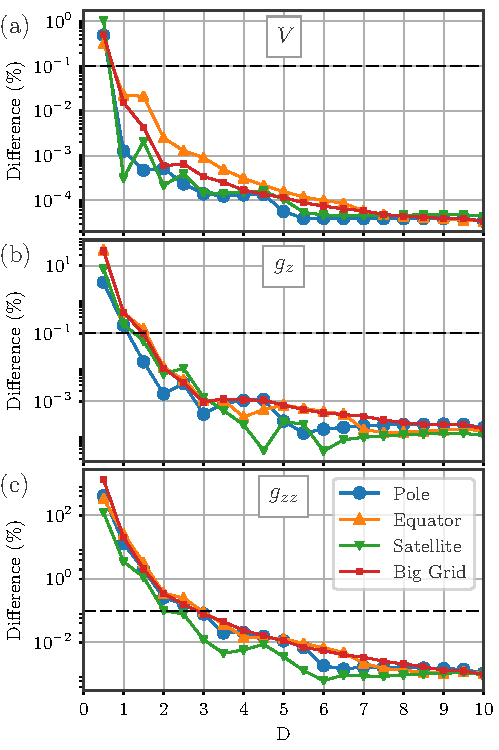
\includegraphics[width=0.9\linewidth]{figures/linear-D-thick.pdf}
\caption{
    Differences between the gravity fields generated by the numerical model and the analytical solution for a thick spherical shell of 35km of thickness with the linear density defined on equation \ref{eq:density-linear}. The computations were performed on the four grids described in Table \ref{tab:grids}, for different values of the distance-size ratio $D$ and without applying the density-based discretization algorithm. If the difference is less than 0.1\%, we consider that the model has achieved an acceptable accuracy for the corresponding value of $D$.
}
\label{fig:D-linear-thick}
\end{figure}


\subsection{Exponential Density}

To test the model in case of an exponential density we proposed the following function:

\begin{equation}
    \rho(r') = A \left( e^{-(r' - R)/b} - 1\right) + 2670 \text{kg/m}^3,
\label{eq:density-exp}
\end{equation}
\noindent where
\begin{equation}
    A =
    (3300 \text{kg/m}^3 - 2670 \text{kg/m}^3)
    \left( e^{( R_2 - R_1 )/b} - 1 \right)^{-1},
\end{equation}

\noindent and the value of $b$ equal to the thickness of the spherical shell we use to perform the test.
In this way, the density function assumes the values of 2670 kg/m$^3$ and 3300 kg/m$^3$ on the shell's outer and inner radii, respectively.
The analytical solution of the gravity potential is easily obtained as the sum the solution for a pure exponential function and the one for an homogeneous spherical shell.

We have performed this test also with a thin and a thick shell of 1 km and 35 km, respectively, without applying the density-based discretization algorithm.
On both cases, the constant $b$ is equal to the thickness of the shell: 1km for the thin shell and 35km for the thick one.
The results can be seen in Figures \ref{fig:D-exp-thin} and \ref{fig:D-exp-thick}.
Once again, the results for $g_{xx}$ and $g_{yy}$ are very similar to the ones obtained for $g_{zz}$, so we exclude them, although, they can be found in the repository.

In the same way we analysed the linear density results, we can summarise that the thin spherical shell presents the more conservative values of the distance-size ratio: $D=1$ for the gravity potential, $D=2$ for its gradient components and $D=8$ for the Marussi tensor components.

\begin{figure}
\centering
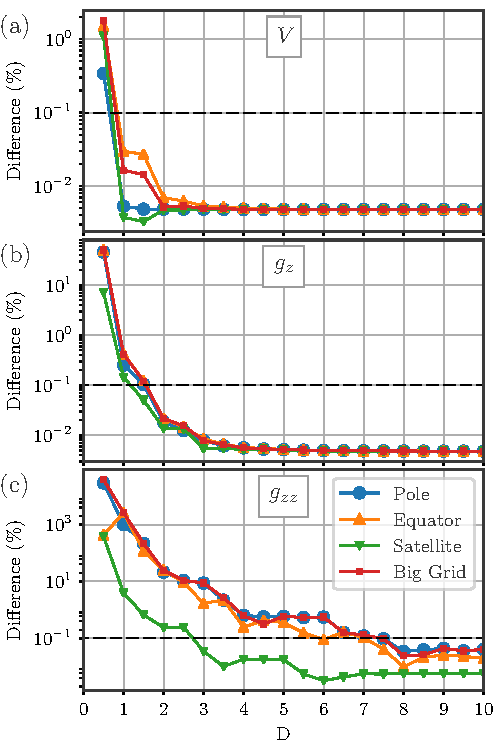
\includegraphics[width=0.9\linewidth]{figures/exponential-D-thin.pdf}
\caption{
    Differences between the gravity fields generated by the numerical model and the analytical solution for a thin spherical shell of 1km of thickness with the exponential density defined on equation \ref{eq:density-exp}. The computations were performed on the four grids described in Table \ref{tab:grids}, for different values of the distance-size ratio $D$ and without applying the density-based discretization algorithm. If the difference is less than 0.1\%, we consider that the model has achieved an acceptable accuracy for the corresponding value of $D$.
}
\label{fig:D-exp-thin}
\end{figure}

\begin{figure}
\centering
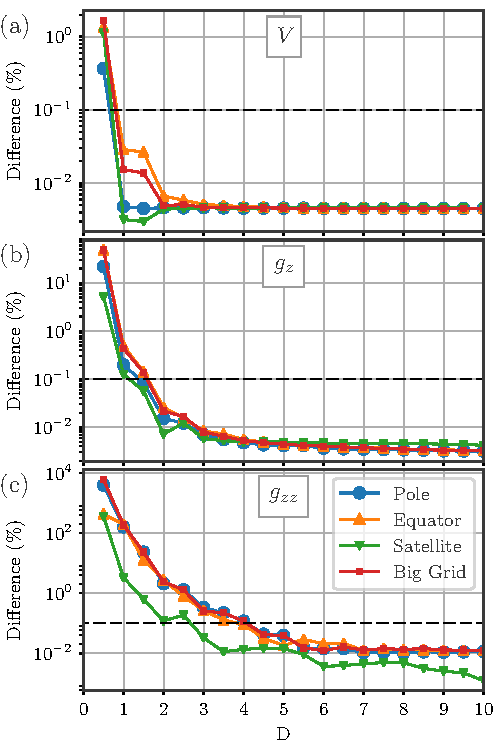
\includegraphics[width=0.9\linewidth]{figures/exponential-D-thick.pdf}
\caption{
    Differences between the gravity fields generated by the numerical model and the analytical solution for a thick spherical shell of 35km of thickness with the exponential density defined on equation \ref{eq:density-exp}. The computations were performed on the four grids described in Table \ref{tab:grids}, for different values of the distance-size ratio $D$ and without applying the density-based discretization algorithm. If the difference is less than 0.1\%, we consider that the model has achieved an acceptable accuracy for the corresponding value of $D$.
}
\label{fig:D-exp-thick}
\end{figure}

Because the constant $b$ controls the variation of the density function, we wanted to test how does the accuracy of the method behaves at different values of $b$ when the density-based discretization algorithm is not applied.
In order to do this we proposed a set of density functions, each one with a different value of $b$.
We computed the difference between the Marussi tensor component $g_{zz}$ generated by the numerical model on the big grid of 30$^\circ\times$30$^\circ$ (see Table \ref{tab:grids}) and the corresponding analytical solution.
These differences were calculated for each proposed density function and for the same set of values of $D$ we have been using on the previous tests, obtaining one curve for each value of $b$.

On Figure \ref{fig:D-exp-power-thin}a we can see the density functions used to perform these tests and its corresponding results on \ref{fig:D-exp-power-thin}b .
Taking into account that lower values of $b$ implies a more varying function, we can see that for high varying functions the numerical model does not perform well: for $b=100$m the difference is almost 100\%.

We can conclude that even when the density-based discretization algorithm is not applied, the numerical approximation performs under the acceptable threshold for values of $b$ greater than the thickness of the shell, i.e. for low density variations.
On the other hand, a density-based discretization algorithm is needed in order to guarantee the accuracy of the approximation in case of a high varying density function.

\begin{figure}
\centering
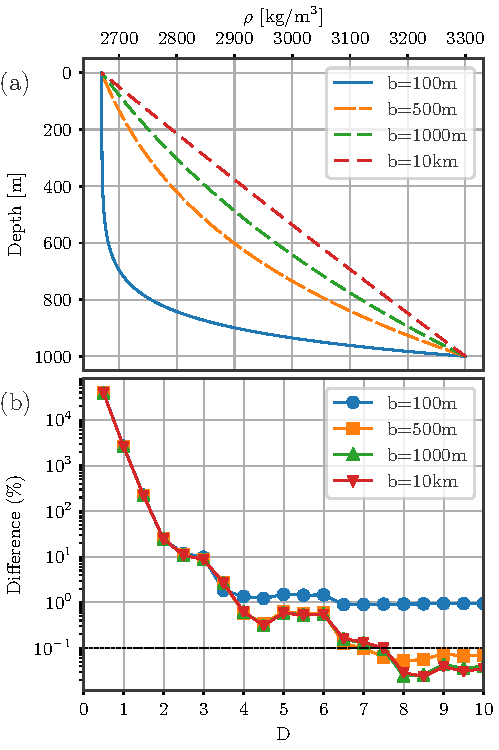
\includegraphics[width=0.9\linewidth]{figures/exponential-b-thin.pdf}
\caption{
    Results of the distance-size ratio determination for different exponential density functions in case of a spherical shell of 1km of thickness.
    (a) Density functions used in the tests, each one with a different value of $b$ and normalised in such way that they reaches a density of 2900kg/m$^{3}$ at the bottom of the shell.
    (b) Differences between the Marussi tensor component $g_{zz}$ generated by the numerical model and the analytical solution for each density function. Each computation was performed on the big grid described in Table \ref{tab:grids}, for different values of the distance-size ratio $D$. If the difference is less than 0.1\%, we consider that the model has achieved an acceptable accuracy for the corresponding value of $D$.
}
\label{fig:D-exp-power-thin}
\end{figure}

\subsection{Discontinuous Density}

As a final case, we performed the same test with a discontinuous density function:

\begin{equation}
    \rho(r') = 
    \begin{cases}
        \rho_A & \text{if} \, R_1 \leq r' < R_c \\
        \rho_B & \text{if} \, R_c \leq r' \leq R_2 \\
    \end{cases}
\label{eq:density-discontinuous}
\end{equation}

\noindent where $\rho_A$ and $\rho_B$ are constant densities, $R_1$ and $R_2$ are the inner and outer radii of the shell, respectively, and $R_c$ is the the radius on which the density change takes place.

The analytical solution for this kind of density is a linear combination of two homogeneous shells with densities $\rho_A$ and $\rho_B$:

\begin{equation}
    V(r) = \frac{4}{3} \frac{\pi G}{r}
    \left[ \rho_A (R_c^3 - R_1^3) +
    \rho_B (R_2^3 - R_c^3) \right]
\end{equation}

Firstly, lets assume a symmetric density function, i.e. $R_c=(R_1 + R_2)/2$ is the centre radius of the shell, and perform the test for a thin shell of 1km of thickness without applying the density-based discretization algorithm.
The results can be seen in Figure \ref{fig:D-discont-sym}.
Once again, we obtain good accuracy for values of $D$ equal to 1, 2 and 8 for the computation of the potential, the gradient components and the Marussi tensor components, respectively.

\begin{figure}
\centering
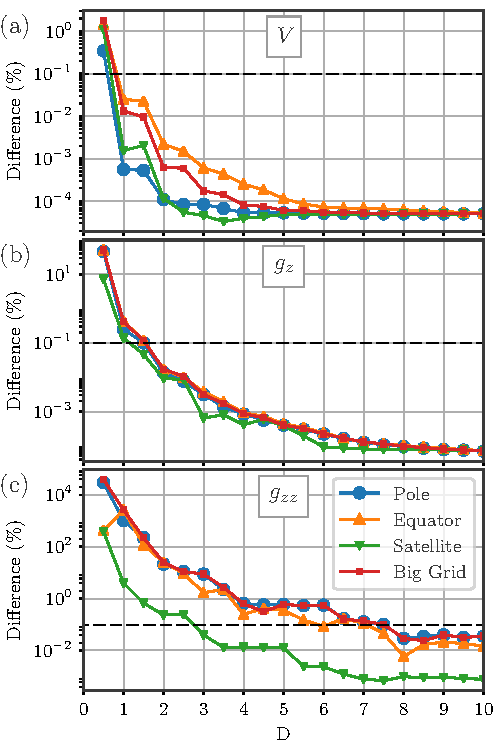
\includegraphics[width=0.9\linewidth]{figures/discontinuous-D-sym.pdf}
\caption{
    Differences between the gravity fields generated by the numerical model and the analytical solution for a thin spherical shell of 1km of thickness with the discontinuous density defined on equation \ref{eq:density-discontinuous} and $R_c$ as the centre radius of the shell. The computations were performed on the four grids described in Table \ref{tab:grids} and for different values of the distance-size ratio $D$. If the difference is less than 0.1\%, we consider that the model has achieved an acceptable accuracy for the corresponding value of $D$.
}
\label{fig:D-discont-sym}
\end{figure}

Secondly, lets assume the same density function from equation \ref{eq:density-discontinuous}, but now with an asymmetrical distribution: $R_c = (R_1 + R_2)/3$, and perform the same test.
We can see its results in Figure \ref{fig:D-discont-asym}: up to $D=10$ the difference between the numerical model and the analytical solution is greater than 10\%, what
leads us to conclude that a density-based discretization algorithm is needed in order to guarantee the accuracy of the model.

\begin{figure}
\centering
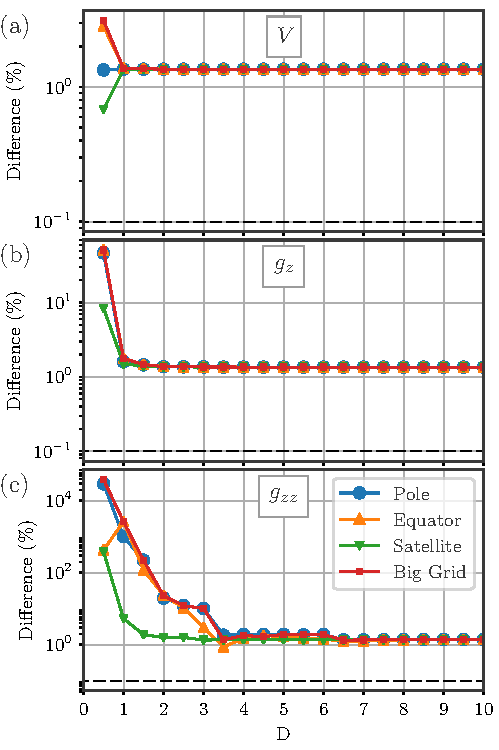
\includegraphics[width=0.9\linewidth]{figures/discontinuous-D-asym.pdf}
\caption{
    Differences between the gravity fields generated by the numerical model and the analytical solution for a thin spherical shell of 1km of thickness with the discontinuous density defined on equation \ref{eq:density-discontinuous} and $R_c=(R_1 + R_2)/3$. The computations were performed on the four grids described in Table \ref{tab:grids} and for different values of the distance-size ratio $D$. If the difference is less than 0.1\%, we consider that the model has achieved an acceptable accuracy for the corresponding value of $D$.
}
\label{fig:D-discont-asym}
\end{figure}


%%%%%%%%%%%%%%%%%%%%%%%%%%%%%%%%%%%%%%%%%%%%%%%%%%%%%%%%%%%%%%%%%%%%%%%%%%%%%%%

\section{Determination of delta ratio}

In the light of the previous results, a density-based discretization algorithm is needed in order to achieve an acceptable accuracy in those cases on which the modified adaptive discretization algorithm is not sufficient to take into account the numerical error due to density variations.

Besides the implementation of this new algorithm, we must determine the maximum value of the delta ratio $\delta$ that produces an accuracy bellow a predefined threshold in order to guarantee the good performance of the numerical model.

To do this we applied a similar methodology used in the determination of the distance-size ratio $D$: we proposed a set of exponential density functions (as the one in equation \ref{eq:density-exp}) with different values of $b$, and computed the difference between the gravity fields generated by the numerical model with the corresponding analytical solution, each time with a different value of $\delta$ ranging from 0.1 to 1 with a step of 0.1.
This tests have been performed for a thin and a thick spherical shell of 1km and 35km of thickness, respectively.

\begin{figure}
\centering
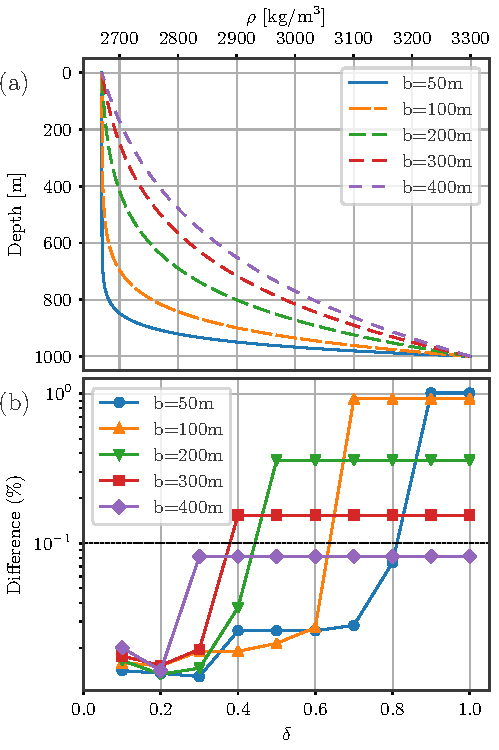
\includegraphics[width=0.9\linewidth]{figures/exponential-delta-thin.pdf}
\caption{
    Results of the delta ratio determination, applied to a thin spherical shell (1km of thickness) with various exponential density functions, each one with different value of $b$.
    (a) Density functions used to perform the test.
    (b) Differences between the numerical model and the corresponding analytical solution for several values of $\delta$ and $b$.}
\label{fig:exponential-delta-thin}
\end{figure}

\begin{figure}
\centering
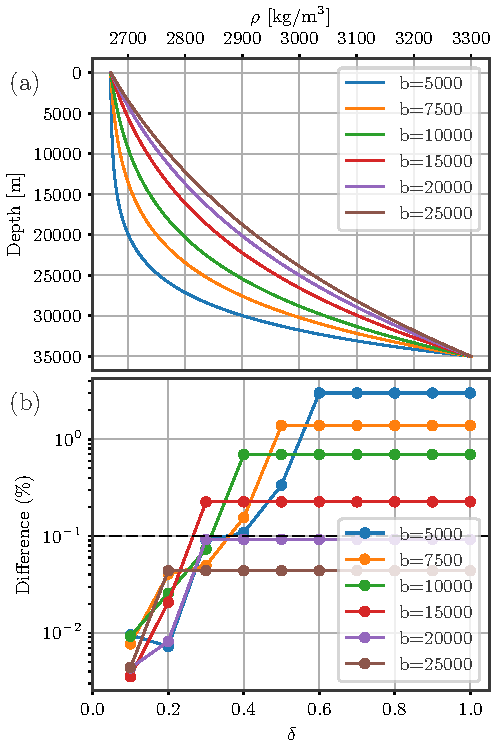
\includegraphics[width=0.9\linewidth]{figures/exponential-delta-thick.pdf}
\caption{
    Results of the delta ratio determination, applied to a thick spherical shell (35km of thickness) with various exponential density functions, each one with different value of $b$.
    (a) Density functions used to perform the test.
    (b) Differences between the numerical model and the corresponding analytical solution for several values of $\delta$ and $b$.}
\label{fig:exponential-delta-thick}
\end{figure}

On Figures \ref{fig:exponential-delta-thin}a and \ref{fig:exponential-delta-thick}a we can see the exponential density functions used on each test for a thin and thick spherical shell, respectively.
While Figures \ref{fig:exponential-delta-thin}b and \ref{fig:exponential-delta-thin}b show their corresponding results.

In the thin shell case we can conclude that a delta equal to 0.3 guarantee an acceptable accuracy under 0.1\% for the entire set of the density functions, while the thick shell case needs at least a delta equal to 0.2.
We will keep the more conservative value of 0.2 as the default value of delta on future computations.

Furthermore, we computed the difference between the numerical model and the analytical solution in case of a discontinuous density (as the one in equation \ref{eq:density-discontinuous} with $R_c = (R_1 + R_2)/3$) using a $\delta = 0.2$.
The result for the $g_{zz}$ component of the Marussi tensor is bellow the 0.1\% threshold, achieving a good performance for this default value of $\delta$.


%%%%%%%%%%%%%%%%%%%%%%%%%%%%%%%%%%%%%%%%%%%%%%%%%%%%%%%%%%%%%%%%%%%%%%%%%%%%%%%

\section{Speed Comparison}

We have recorded the computation times for the gravity potential, the gradient component $g_z$ and the Marussi tensor component $g_{zz}$ generated by a single tesseroid model with homogeneous ($\Delta t_\text{homogeneous}$) and variable ($\Delta t_\text{variable}$) density at different heights. Then we plotted the ratio between these computation times (see Figure \ref{fig:speed-comparison}): 

\begin{equation}
    \text{Computation Times Ratio} =
        \frac{\Delta t_\text{variable}}{\Delta t_\text{homogeneous}}
    \label{eq:computation-times-ratio}
\end{equation}

From these results we can conclude that the homogeneous density code is up to twice faster than the new variable density algorithm for lower heights. However, the computation times ratio gets lower at greater heights, due to the reduction of the divisions made by the adaptive discretization algorithm. In summary, the new variable density code is fast enough to perform the calculations of a real model in a few minutes. \todo{real, esta bien la expresion?}

\begin{figure}
\centering
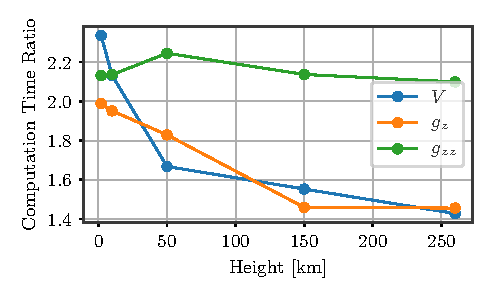
\includegraphics[width=0.9\linewidth]{figures/speed-comparison.pdf}
\caption{Computation times ratio between a single tesseroid model with variable and with homogeneous density at different heights, defined in equation \ref{eq:computation-times-ratio}.}
\label{fig:speed-comparison}
\end{figure}


%%%%%%%%%%%%%%%%%%%%%%%%%%%%%%%%%%%%%%%%%%%%%%%%%%%%%%%%%%%%%%%%%%%%%%%%%%%%%%%

\section{Example with real data}

Besides all the tests we have carried out on the new code, we intend to show a forward modelling example with real data.
In order to do that we have chosen the Neuqu\'en Basin: a sedimentary basin located to the east of the Andes, between 32$^\circ$S and 40$^\circ$S latitude (see Figure \ref{fig:neuquen-basin}a), that includes continental and marine siliciclastics, carbonates and evaporites accumulated over the Jurassic and the Cretaceous constituting a stratigraphic record up to 5000m of depth \citep{Howell2005}.

\begin{figure*}
\centering
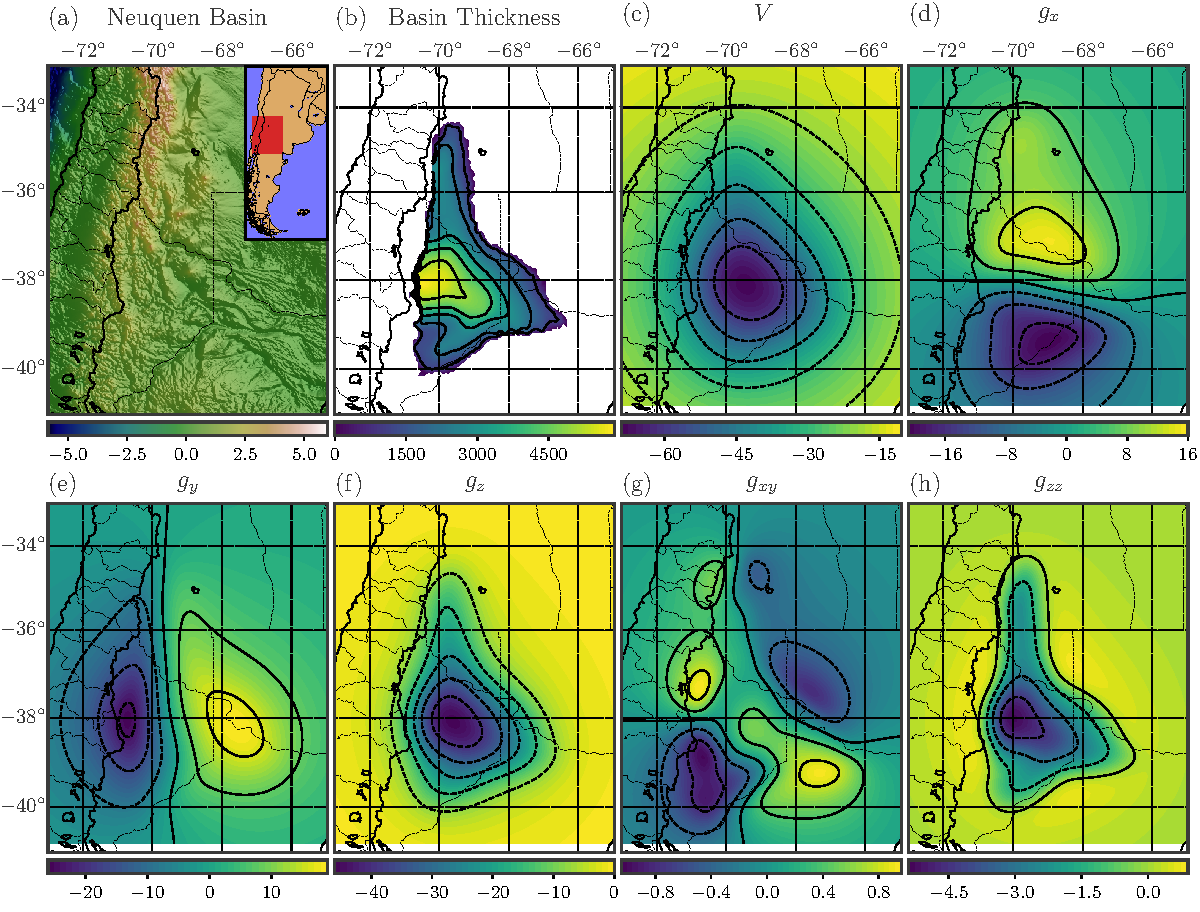
\includegraphics[width=\linewidth]{figures/neuquen-basin.pdf}
\caption{(a) Topography of Neuqu\'en Basin (in km),
         (b) Thickness of the sedimentary basin (in meters),
         (c)-(h) Computed gravity fields: potential $V$ (in J/kg), gradient components $g_x$, $g_y$ and $g_z$ (in mGal) and Marussi tensor components $g_{xy}$ and $g_{zz}$ (in Eötvös), calculated at 50km of height over the ellipsoid.}
\label{fig:neuquen-basin}
\end{figure*}

The thickness of the sediment pack was obtained from \citet{Heine2007}.
We managed to produce a regular grid with a resolution of 0.05$^\circ$ on both longitude and latitude directions with one value of thickness on each node (see Figure \ref{fig:neuquen-basin}b).

In order to compute the gravity fields generated by this basin we created a mesh of tesseroids, each one located on one of the nodes of the grid, with dimensions of 0.05$^\circ$ $\times$ 0.05$^\circ$ and depth equal to the thickness of the basin on the corresponding node.

We must also define a density function for the entire model.
\citet{Sigismondi2012} proposed a minimum and a maximum density for the Neuqu\'en basin of 275kg/m$^3$ and 412kg/m$^3$, respectively.
So we have chosen, for this specific example, a linear density that assumes the minimum value on the surface and the maximum at 5858m, i.e. the bottom of the basin.

We have finally computed the gravity potential $V$, the gradient components $g_x$, $g_y$ and $g_z$, and the Marussi tensor components $g_{xy}$ and $g_{zz}$ on a computation grid of 159$\times$163 nodes with a 0.05$^\circ$ spacing on both longitude and latitude directions at a 50km height over the reference ellipsoid.
The resulting gravity fields can be seen in Figures \ref{fig:neuquen-basin}c-h.
We have excluded the other components of the Marussi tensor from the Figure, although they have also been computed and can be found in the repository.


%%%%%%%%%%%%%%%%%%%%%%%%%%%%%%%%%%%%%%%%%%%%%%%%%%%%%%%%%%%%%%%%%%%%%%%%%%%%%%%

\section{Conclusions}

We have developed a Python library that allows us to perform forward gravity computations using tesseroids with variable density in depth.
The code numerically approximates the integral that defines the gravity potential, its gradient and the Marussi tensor through the Gauss-Legendre Quadrature (GLQ).
It essentially consists in approximating the gravity fields of the tesseroids with the effect of point masses located on the scaled nodes of the Legendre polynomials.
We state that this method it's well suited to approximate the effect of tesseroids with arbitrary densities, in contrast with the ones that involve Taylor series expansion.

Instead of enhancing the accuracy of the method by increasing the order of the GLQ on each integration, we make use of the preexisting modified adaptive discretization algorithm and a new density-based discretization algodithm.

The former one divides the tesseroid by half if the ratio of the distance to the computation point and its size is lower than a predefined distance-size ratio $D$.
We can summarise that $D$ controls the accuracy of the method: a higher value of $D$ generates more divisions of the tesseroids, thus more point masses, what leads to a more precise approximation.
Nevertheless it is not sufficient to guarantee the accuracy of the method in case of specific density functions as a highly variable exponential or some discontinuous functions.

For this reason we developed a density-based discretization algorithm that divides the tesseroid on the radius at which the \emph{maximum variation} of the density function takes place, only if a inequation that relates this \emph{maximum variation} with a predefined delta ratio $\delta$ holds.
Therefore the number of subdivisions is indirectly controlled by this delta ratio $\delta$, and thus the accuracy of the computation.

Because there is no direct relation between the values of $D$ and $\delta$ and the error of the computation, we had to empirically determine the minimum value of $D$ and the maximum value of $\delta$ that produce an acceptable accuracy for each gravity field.

The distance-size ratio determinations have been made through the comparison of the numerical approximations with the analytical solutions for the a spherical shell with variable density, which had to be analytically obtained.
From the wide range of possible density variations, we've chosen a linear, an exponential and a discontinuous density functions.
These comparisons have been made without applying the density-based discretization algorithm in order to isolate the other one.
The tests over the first two functions have shown that a value of $D$ equal to 1, 2 and 8 must be used in the calculation of the gravity potential, its gradient components and the components of the Marussi tensor, respectively, in order to achieve an accuracy bellow 0.1\%.
On the other hand we have found a limitation of this algorithm working on its own in case of highly varying exponential functions and in some cases of discontinuous density.

Nevertheless, the density-based discretization algorithm have shown that a value of $\delta = 0.2$ (together with the previously obtained default values of $D$) guarantees a good accuracy on those cases on which the modified adaptive discretization algorithm does not achieve it on its own.

Finally, we have shown a real data example: we have computed the gravity fields generated by the Neuqu\'en sedimentary basin through a tesseroid model with linear increasing density with depth on a regular grid at 50km height.


%%%%%%%%%%%%%%%%%%%%%%%%%%%%%%%%%%%%%%%%%%%%%%%%%%%%%%%%%%%%%%%%%%%%%%%%%%%%%%%

\section{Acknowledgments}

We are indebted to the developers and maintainers of the open-source
software without which this work would not have been possible.

%%%%%%%%%%%%%%%%%%%%%%%%%%%%%%%%%%%%%%%%%%%%%%%%%%%%%%%%%%%%%%%%%%%%%%%%%%%%%%%

\bibliographystyle{gji}
\bibliography{bibtex/references}

\end{document}
